\documentclass[a4paper,11pt]{article}

\usepackage[T1]{fontenc}
\usepackage[utf8]{inputenc}
\usepackage{csquotes}
\usepackage[authoryear,round]{natbib}
\usepackage[french]{babel}
\usepackage{geometry}
\usepackage{hyperref}
\usepackage{xcolor}
\usepackage{graphicx}
\usepackage{fancyhdr}
\usepackage{array}
\usepackage{booktabs}
\usepackage{enumitem}
\usepackage{tikz}
\usetikzlibrary{positioning,arrows.meta,shapes.geometric}
\usepackage[expansion=false]{microtype}
\usepackage{amsmath}
\usepackage{float}

\addto\captionsfrench{\renewcommand{\contentsname}{Sommaire}}

\geometry{
  a4paper,
  left=2.5cm,
  right=2.5cm,
  top=2.5cm,
  bottom=2.5cm,
  centering
}

\setlength{\headheight}{15pt}
\setlength{\headsep}{12pt}
\hypersetup{hidelinks}

\renewcommand{\sectionmark}[1]{\markright{#1}}
\fancyhf{}
\fancyhead[R]{\nouppercase{\rightmark}}
\fancyfoot[C]{\thepage}
\renewcommand{\headrulewidth}{0pt}
\renewcommand{\footrulewidth}{0.4pt}
\fancypagestyle{plain}{%
  \fancyhf{}
  \fancyhead[R]{\nouppercase{\rightmark}}
  \fancyfoot[C]{\thepage}
  \renewcommand{\headrulewidth}{0pt}
  \renewcommand{\footrulewidth}{0.4pt}
}


\newcommand{\titreEtude}{Développement d'un outil permettant le traitement et l'insertion des archives numériques sur Geofoncier au sein d'un cabinet de Géomètre-Expert}
\newcommand{\auteur}{TRAVAILLÉ Adrien}
\newcommand{\specialite}{INSA Strasbourg - Spécialité Topographie}
\newcommand{\structure}{Cabinet de Géomètre-Expert (structure d'accueil : GEO-SIAPP)}
\newcommand{\encadrement}{Encadrant : Mathieu KOEHL}
\newcommand{\dateRapport}{Mai 2026}

\title{\textbf{Rapport d'activités de mi-parcours (PFE)}\\[0.4em]\large \titreEtude}
\author{\auteur\\\specialite\\\structure\\\encadrement}
\date{\dateRapport}

\begin{document}

\begin{titlepage}
  \thispagestyle{empty}
  \noindent% <-- important : le % supprime l'espace parasite
  \begin{minipage}[c]{0.45\textwidth}
    
\includegraphics[height=2.8cm]{Logo_INSAStrasbourg.jpg}
  \end{minipage}% <-- important : supprime le saut de ligne
  \hfill
  \begin{minipage}[c]{0.45\textwidth}
    \raggedleft
    
\includegraphics[height=2.8cm]{Geosiapp.jpg}
  \end{minipage}

  \vspace{4em}
  \begin{center}
    {\Huge\bfseries\sffamily Rapport d'activités mi-parcours\par}
    \vspace{0.6em}
    {\Large\bfseries\sffamily (PFE)\par}
    \vspace{1em}
    
    {\rule{0.35\linewidth}{1pt}\par}
    \vspace{2.5em}
    
    % Mise en valeur du titre : en gras, plus grand, et bien espacé
    {\LARGE\bfseries \titreEtude\par}
    
    \vspace{3.5em}
    {\large \textbf{\auteur}\par}
    \vspace{0.5em}
    {\large \specialite\par}
    {\large \structure\par}
    {\large \encadrement\par}
    \vfill
    {\large \dateRapport\par}
  \end{center}
\end{titlepage}

\cleardoublepage
\pagenumbering{gobble}
\pdfbookmark[1]{\contentsname}{toc}
\tableofcontents
\begin{tikzpicture}[remember picture,overlay]
  \node [yshift=2cm] at (current page.south) {\footnotesize \textit{Note : Le texte de ce document a fait l'objet d'une relecture et d'une reformulation par intelligence artificielle, dans un souci de lisibilité.}};
\end{tikzpicture}

\clearpage
\pagestyle{fancy}
\pagenumbering{arabic}
\setcounter{page}{1}



\begin{center}

\vspace{1em}

\textbf{Titre de l'étude :} \titreEtude.\\[0.5em]
\end{center}

\vspace{1em}

\section{Définition, cadrage et objectifs}

\subsection{Contexte juridique et importance des archives}
La profession de géomètre-expert est réglementée, tout comme la gestion de la donnée foncière qu'elle produit et dont elle dispose de l'exclusivité. Selon l'article 55 du décret n°96-478 du 31 mai 1996 (portant sur les devoirs professionnels), le géomètre-expert a l'obligation de conserver et de tenir à jour les archives et documents topographiques fixant les limites des biens fonciers. Ces documents (procès-verbaux de bornage, plans de division, documents d'arpentage) sont alors classifiés et conservés par les cabinets.

Lorsqu'une nouvelle mission foncière est confiée au cabinet, la première étape pour l'opérateur consiste à effectuer une recherche ou une reconnaissance des limites, dans le but d'appliquer un éventuel document déjà produit. Pour ce faire, il se connecte systématiquement sur \textbf{Géofoncier}, le portail national de l'Ordre des géomètres-experts, afin de vérifier si une opération foncière a déjà eu lieu sur les parcelles concernées ou à proximité. Si le portail indique l'existence d'une intervention passée (ou si les propriétaires voisins mentionnent l'existence d'un ancien plan lors des premiers échanges), l'opérateur doit impérativement en retrouver la trace. S'il s'agit d'un dossier récent, le plan peut souvent être téléchargé directement depuis le portail. En revanche, si l'opération est ancienne, il doit rechercher physiquement dans le stock d'archives du cabinet, ou contacter le géomètre-expert détenteur de l'archive pour en obtenir une copie.

\subsection{Le besoin d'automatisation chez Géo-Siapp}
Le cabinet Géo-Siapp dispose d'un fonds d'archives très important, accumulé au fil des décennies (estimé pour la période 1959-2007) et réparti sur ses différentes agences en Ardèche. Ces dossiers sont extrêmement hétérogènes : plans papiers manuscrits, registres anciens, ou vieux documents scannés sous forme d'images. 

Si les plans modernes sont aujourd'hui numériques et versés sur Géofoncier, la majorité du passif (les archives historiques du cabinet) n'est ni indexée, ni géo-référencée, encore moins versée. Lorsqu'un opérateur cherche une donnée ancienne pour une nouvelle mission, la recherche manuelle dans ces papiers ou dans des dossiers informatiques mal classés est une tâche très chronophage.

L'objectif de ce projet est donc de concevoir un système automatisé capable d'analyser ces archives brutes numérisées pour en extraire les informations clés (la commune, la date, le numéro de document d'arpentage...). Ce système doit permettre de structurer l'information pour générer automatiquement des dossiers locaux, et préparer un versement massif sur la plateforme Géofoncier. Pour garantir la qualité de la donnée foncière, il est également nécessaire que chaque étape d'extraction soit vérifiable par les opérateurs grâce à une interface de validation, permettant de corriger les erreurs de la machine.

La difficulté principale de cette démarche réside dans la grande variabilité des documents, une problématique largement étudiée dans le domaine de la reconnaissance de texte manuscrit (HTR) \citep{alkendi_advancements_2024}. L'hétérogénéité des mises en page, la dégradation du papier, et la complexité des écritures des anciens géomètres-experts exigent de dépasser la simple lecture optique (OCR) et d'utiliser une chaîne de traitement faisant appel à l'intelligence artificielle.

Le schéma ci-dessous résume la trame du projet :
\begin{figure}[H]
  \centering
  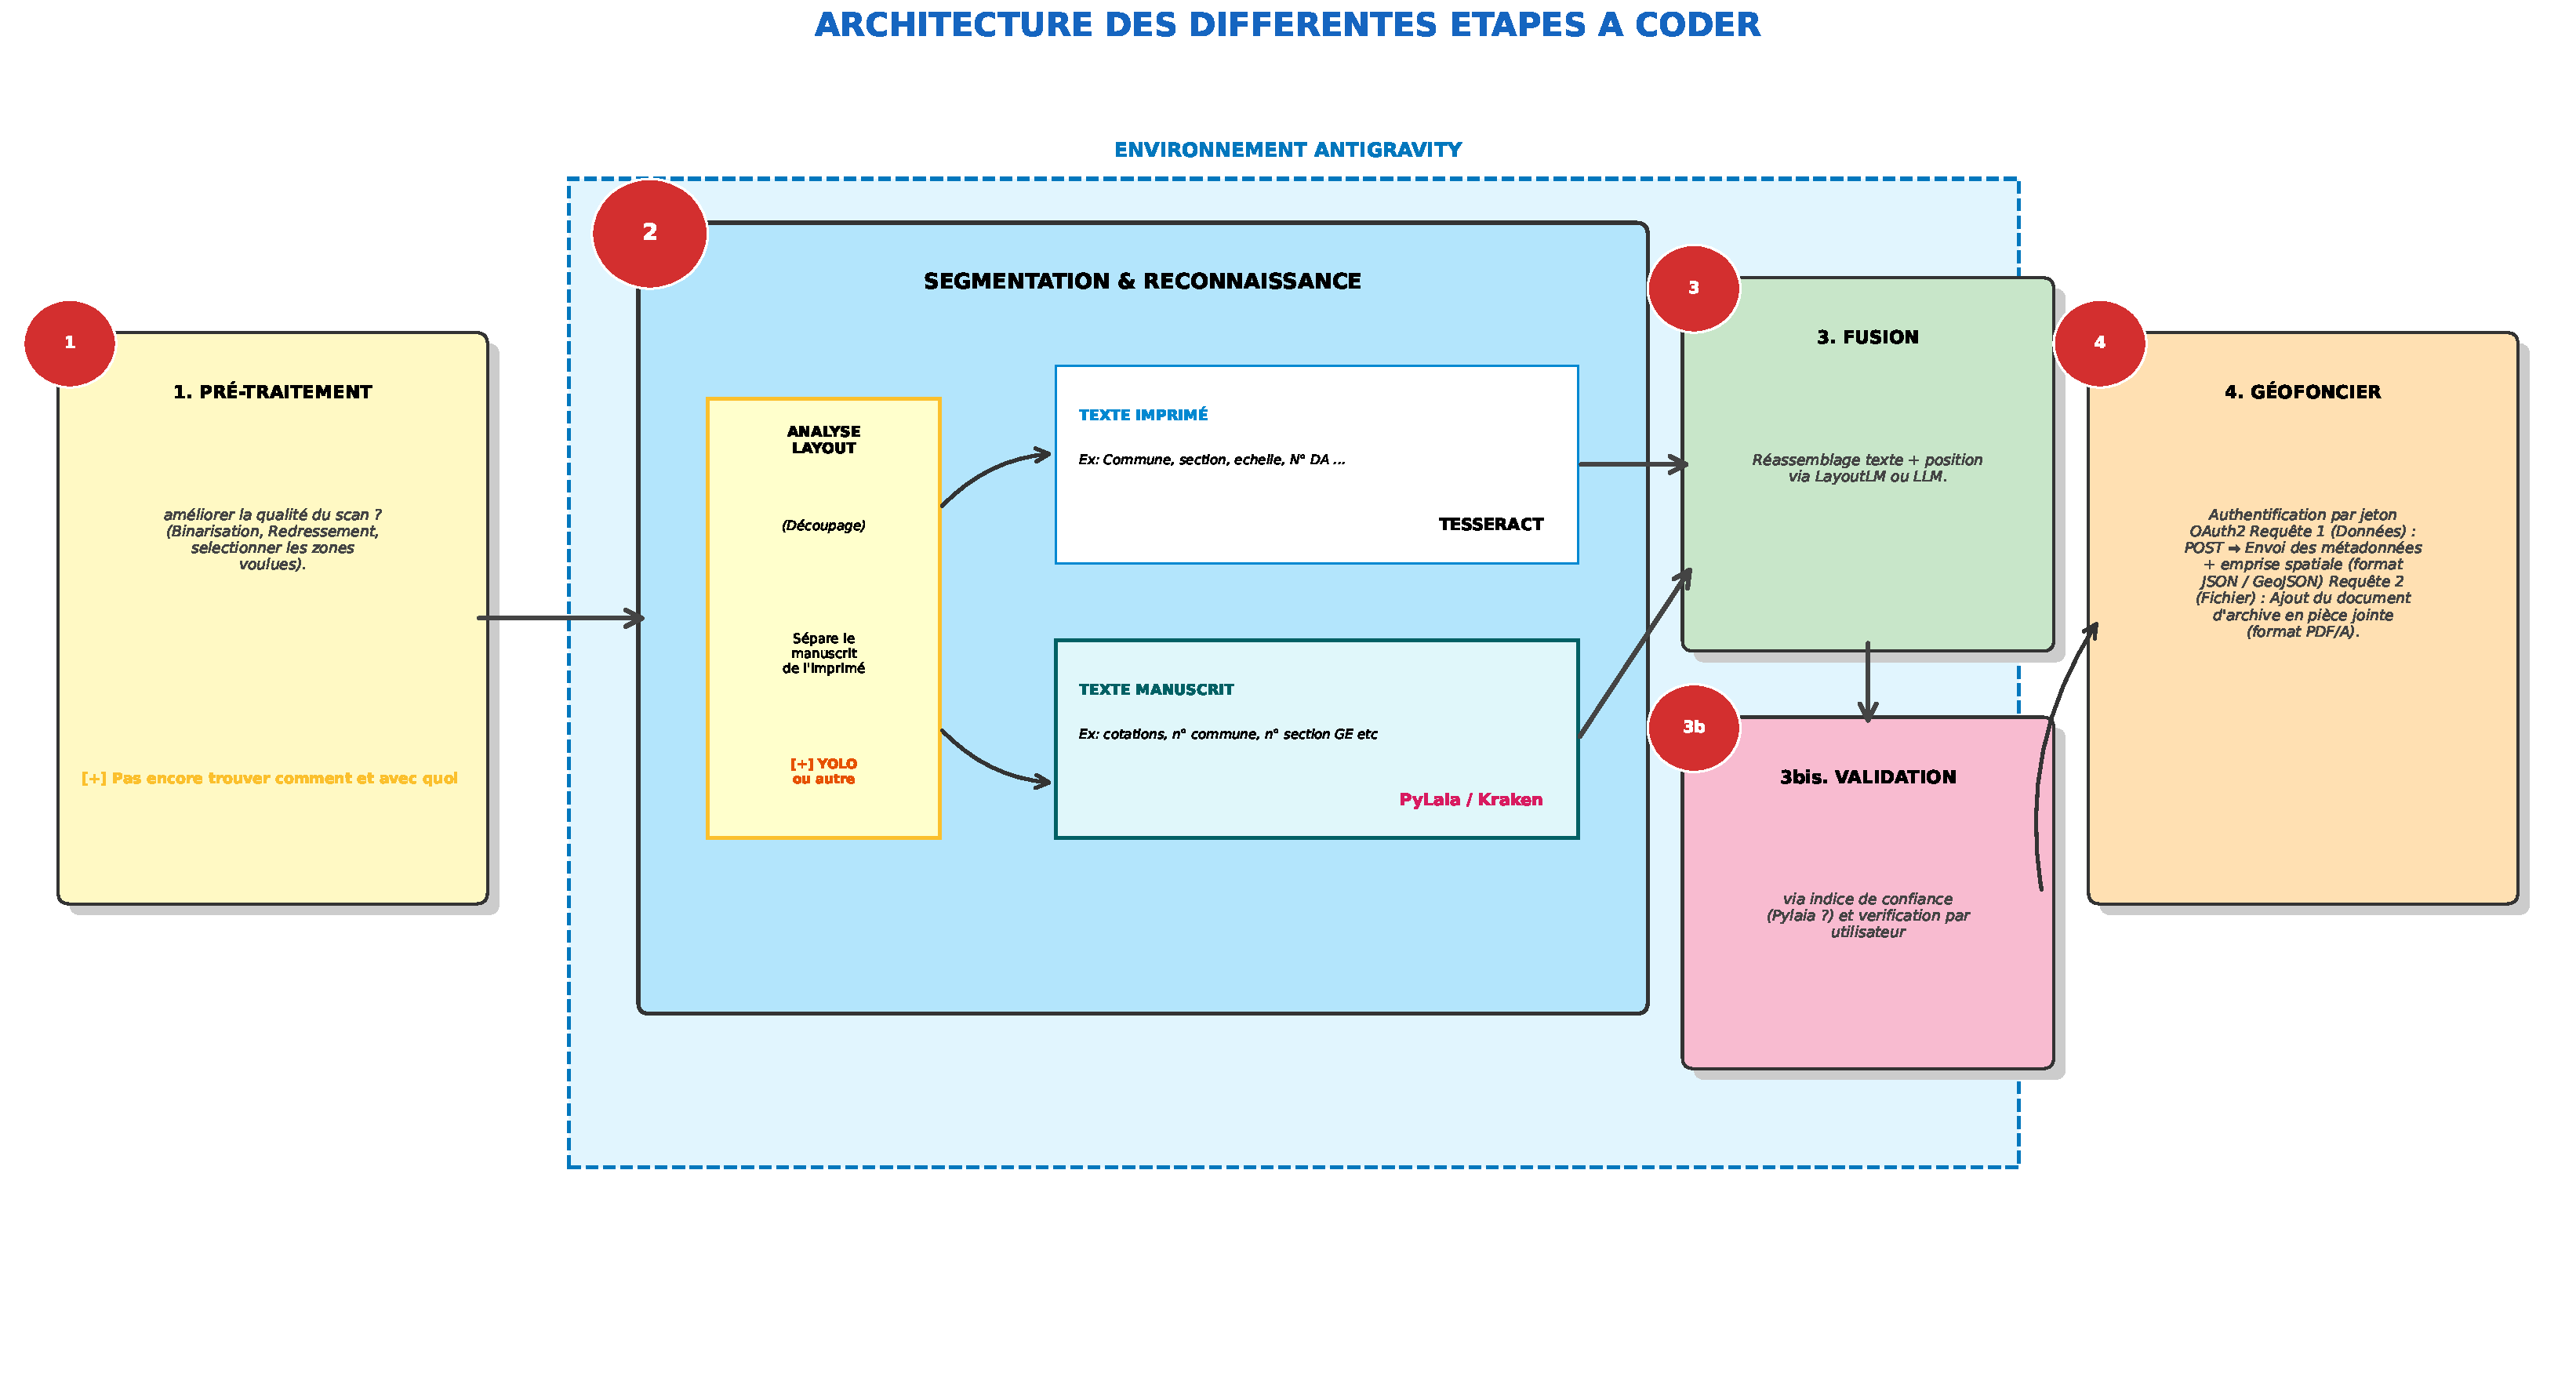
\includegraphics[width=1\textwidth]{img/architecture_pfe_complet.pdf}
  \caption{Architecture globale du projet (lisible en annexe)}
  \label{fig:architecture_pfe}
\end{figure}


L'architecture de ce système de traitement est conçue autour de quatre étapes. Le projet s'organise autour d'un fichier central en language de programmation python(\texttt{main.py}) :

\begin{itemize}[leftmargin=1.2em]
  \item \textbf{Étape 1 : Tri et classification automatique.} Le script principal (\texttt{main.py}) analyse le document d'entrée pour identifier sa nature (plan vectoriel récent, plan numérisé, ou registre manuscrit) et le rediriger vers le module d'extraction adéquat. Cette logique d'orientation est en place, mais les paramètres de classification pour certains cas limites restent à peaufiner.
  
  \item \textbf{Étape 2 : Extraction des données.} Le programme isole les informations ciblées. Pour les plans cadastraux récents, un module dédié (\texttt{modern\_plan\_extractor.py}) est mis en place. En revanche, pour les documents anciens, l'extraction repose sur des modèles d'intelligence artificielle (HTR) dont les réglages doivent encore être peaufinés face aux écritures les plus dégradées.
  
  \item \textbf{Étape 3 : Contrôle et validation.} Une fois les données extraites, le script de vérification (\texttt{semantic\_ocr\_engine.py}) effectue une première correction (croisement INSEE, formatage des dates). L'opérateur utilise ensuite une interface visuelle (\texttt{app\_validation.py}) pour valider ou corriger la donnée. L'outil enregistre les interventions manuelles dans le répertoire \texttt{writer\_styles/} pour améliorer les prochaines lectures. Cette étape est fonctionnelle.
  
  \item \textbf{Étape 4 : Formatage et versement Géofoncier.} Les données extraites (fichiers CSV placés dans le dossier \texttt{outputs/}) serviront à générer des dossiers locaux et seront envoyées via l'API Géofoncier pour créer la pastille sur le portail. Cette étape n'est pas encore développée et constitue l'objectif de la suite de l'étude.
\end{itemize}

\subsection{Arborescence technique du projet}
Le projet a été découpé en plusieurs \enquote{branches} distinctes. Voici la structure actuelle de l'outil :

\begin{figure}[H]
\begin{verbatim}
Projet_PFE/
|-- main.py # Cœur du programme 
|-- modern_plan_extractor.py # Branche dédiée aux plans les plus récents de la période 
|-- semantic_ocr_engine.py # Branche de vérification 
|-- app_validation.py # Interface visuelle pour l'opérateur (Streamlit)
|-- outputs/ # Dossier contenant tous les résultats générés
| |-- log_exec.txt # Historique et traçabilité de toutes les actions
| |-- *_resultats_nom_doc_entree.csv # Tableaux de données prêts pour Geofoncier
|-- writer_styles/ # Mémoire des corrections apportées par l'opérateur
\end{verbatim}
\caption{Schéma de l'arborescence et des modules du projet}
\end{figure}

\subsection{Périmètre et contraintes à mi-parcours}

Le périmètre d'entrée englobe donc de nombreux types de documents différents, allant du document PDF vectoriel récent aux images scannées (raster) de qualité parfois médiocre, formant des lots d'archives non homogènes. En sortie, le système doit générer des données toujours identiques (fichiers CSV, JSON ou Excel), accompagnées de preuves visuelles pour le contrôle, comme des images annotées. La validation par un opérateur reste indispensable pour traiter les cas les plus ambigus, ou mal écrits.

Ce travail est toutefois soumis à certaines contraintes. D'une part, la dégradation des documents sources (bruit numérique, compression, mauvaise rotation, faible contraste, mauvaise écriture) complique la tâche de segmentation et de lecture. D'autre part, la variabilité des mises en page, qu'il s'agisse de documents en tableau pour des livrets anciens ou de plans cadastraux plus récents, demande une analyse différente en fonction du type de document. L'étude se portera ainsi uniquement sur des entités définies (communes, dates, numéro du document d'arpentage), imposant une recherche d'information sur le document pour y trouver les informations voulues. L'arborescence du projet ainsi que les exécutables doivent pouvoir être déployés sur un environnement Windows classique, via un outillage accessible aux opérateurs et assez simple d'utilisation.

\subsection{Objectifs initiaux, évolutions et options retenues}
Au commencement de l'étude, l'objectif était de développer un programme unique capable de lire n'importe quel type d'archive d'une traite : ouverture du fichier, découpage des zones de texte, transcription automatique par un seul moteur classique (OCR) puis extraction des mots clés. L'idée était ensuite de vérifier ces données avec des bases de référence (comme la liste officielle des communes) et de proposer une interface pour que l'opérateur puisse valider le tout manuellement \citep{beatrice_challenges_2023, stokes_partage_nodate}.

Cependant, en confrontant ce système aux archives Géo-Siapp, les objectifs ont dû évoluer. Il est vite apparu qu'utiliser un moteur OCR universel et unique était une option non viable (non retenue au final), il n'était pas assez performant sur les écritures des anciens géomètres-experts ou sur des images trop dégradées. La première décision a donc été de séparer le traitement pour s'adapter au type de document.

Pour les plans cadastraux modernes, l'option retenue est d'utiliser directement l'agencement visuel de la page pour trouver la bonne information, ce qui s'avère bien plus rapide et fiable qu'une lecture complète du texte. Pour les registres anciens et manuscrits, le défi est tout autre \citep{tarride_improving_2024}. L'option d'une transcription textuelle classique a été définitivement écartée au profit d'une méthode testant de multiples hypothèses de lecture en parallèle, notamment via l'utilisation de petits modules d'intelligence artificielle comme GLiNER. Ce modèle léger a été choisi car il comprend le contexte de la phrase : il est capable de repérer si un mot correspond à une commune ou une date. Cela permet d'éviter de bloquer la chaîne d'extraction lorsqu'une information n'est pas remplie ou si le moteur OCR n'est pas sûr de sa transcription.

Enfin, face aux cas les plus illisibles, l'étude s'est réorientée vers l'intégration de modèles d'Intelligence artificielle plus performants (Modèles Vision-Langage ou VLM). Ces modèles n'interviennent qu'en dernier recours pour trancher un doute, afin de garantir à l'opérateur final la proposition d'extraction la plus pertinente possible, tout en intervenant que localement.

\section{Résultats et synthèse de l'étude bibliographique}

L'étude bibliographique a été importante pour orienter les choix architecturaux du projet. Les recherches récentes démontrent sans équivoque que le traitement des documents anciens et de leurs mises en page complexes (tableaux, formulaires, plans) nécessite une combinaison d'approches, allant de la simple détection de zones aux modèles d'intelligence artificielle avancés \citep{alkendi_advancements_2024}. 

\subsection{Le défi de la reconnaissance de texte manuscrit (HTR)}
Contrairement aux documents modernes générés numériquement, les registres et plans cadastraux anciens présentent d'importantes variations visuelles et structurelles. Comme le soulignent \citet{stokes_partage_nodate} et \citet{chague_htr-united_nodate}, la reconnaissance de texte manuscrit (HTR) est fortement dépendante de la qualité des données d'entraînement. Les moteurs d'extraction classiques basés uniquement sur la reconnaissance optique de caractères (OCR) affichent très souvent leurs limites face aux écritures anciennes ou aux documents dégradés par le temps. Pour contrer ces problèmes, plusieurs études récentes recommandent l'utilisation d'outils complémentaires comme des modèles de langage statistiques couplés à PyLaia, qui est un moteur de reconnaissance de texte manuscrit open-source, basé sur l'apprentissage profond (Deep Learning) \citep{tarride_improving_2024} ou des procédés hybrides intégrant une correction via des bases de données historiques \citep{sang_ree-hdsc_2024}. Par ailleurs, pour des pages manuscrites, l'adoption d'un vocabulaire contrôlé tel que SegmOnto, un outil de segmentation de texte manuscrit \citep{gabay_segmonto_nodate} permet de rendre la segmentation et le découpage des pages plus efficace.

\subsection{Analyse comparative des modèles de détection}
Pour l'extraction spécifique des mots-clés (communes, numéros de document d'arpentage), de nombreux outils et modèles de détection sont disponibles. Ces derniers vont des approches les plus simples aux plus complexes, variant en précision, temps de calcul et exigences de qualité pour le scan. Les architectures basées sur l'analyse conjointe du texte et de la topologie de la page, comme LayoutLM \citep{xu_layoutlm_2020} et ses évolutions \citep{luo_layoutllm_2024}, offrent des performances optimales pour classifier et extraire des informations, y compris sur des formats spécialisés comme ici. Des comparatifs récents avec d'autres modèles multimodaux, comme Donut, confortent l'avantage des architectures orientées "Layout" \citep{bajrami_comprehensive_2023}. De son côté, la détection purement visuelle et géométrique a été considérablement renforcée par l'évolution des algorithmes YOLO \citep{jiang_review_2022}.

Afin de choisir entre ces différentes technologies, une synthèse comparative (Tableau \ref{tab:comparatif_modeles}) a été réalisée en fonction des critères de précision (face au bruit de l'OCR), de temps de traitement, et de faisabilité de déploiement en local au sein de l'environnement du cabinet.

\begin{table}[H]
\centering
\renewcommand{\arraystretch}{1.5}
\resizebox{\textwidth}{!}{%
\begin{tabular}{|>{\raggedright\arraybackslash}p{4cm}|>{\raggedright\arraybackslash}p{4.5cm}|>{\raggedright\arraybackslash}p{4.5cm}|>{\centering\arraybackslash}p{2.5cm}|}
\hline
\textbf{Technologie} & \textbf{Avantages} & \textbf{Inconvénients} & \textbf{Temps de traitement} \\ 
\hline
\hline
\textbf{Expressions Régulières (Regex)} & Facilité de mise en place. Aucune exigence matérielle. & Taux d'erreurs de plus de 40\% dès que l'OCR varie d'un caractère. & Très rapide ($<$ 0.1s) \\ 
\hline
\textbf{OCR par gabarit (Template Matching)} & Très efficace pour des formulaires figés ou des registres standardisés. & Incapable de s'adapter au moindre décalage spatial (scan de travers, marges variables). & Très rapide ($<$ 0.1s) \\ 
\hline
\textbf{NLP Classique (NER SpaCy, etc.)} & Bonnes performances sur du texte propre. Très léger en mémoire. & Très vulnérable aux fautes d'orthographe générées par l'OCR (sensibilité au bruit numérique). & Rapide ($\sim$ 0.2s) \\ 
\hline
\textbf{Modèles visuels (YOLO)} \newline \citep{jiang_review_2022} & Excellente détection spatiale des blocs (en-têtes, cases). Robuste aux variations de fond de l'image. & N'extrait pas le texte lui-même, nécessite un traitement OCR supplémentaire par la suite. & Rapide ($\sim$ 0.5s) \\ 
\hline
\textbf{Modèles "Layout" (LayoutLM, Donut)} \newline \citep{xu_layoutlm_2020, bajrami_comprehensive_2023} & Bonne précision: ils comprennent simultanément la géométrie de la page et le sens du texte. & Lourdeur de calcul. Nécessite une grande quantité de RAM et un processeur graphique (GPU) dédié. & Modéré ($\sim$ 2 à 5s) \\ 
\hline
\textbf{Modèles sémantiques (GLiNER)} \newline \citep{zaratiana_gliner_2024} & Analyse contextuelle robuste au bruit de l'OCR. Modèle léger fonctionnant hors-ligne sur CPU. & Limité à l'extraction de mots et entités. Ne perçoit pas la structure visuelle du plan. & Rapide ($\sim$ 1s) \\ 
\hline
\textbf{Modèles Vision-Langage (VLM / LLM)} \newline \citep{xu_layoutlm-critic_2022} & Capacités de raisonnement et de correction d'erreurs (joue le rôle d'arbitre ou de \enquote{troisième avis}). & Extrêmement coûteux en ressources informatiques et en temps. Risques d'halluciner. & Lent ($>$ 10s) \\ 
\hline
\end{tabular}%
}
\caption{Comparaison des technologies d'extraction et de détection pour les documents d'archives}
\label{tab:comparatif_modeles}
\end{table}

\subsection{Choix retenus}
Suite à cette comparaison, il s'est avéré que certaines de ces solutions étaient insuffisantes pour répondre aux besoins du cabinet. Le recours exclusif à des algorithmes comme LayoutLM a dû être écarté à cause de leurs exigences, incompatibles avec le matériel informatique du cabinet, pas forcément des plus puissants. 

Le choix s'est donc porté sur un mixte : 
\begin{itemize}[leftmargin=1.2em]
  \item \textbf{Pour la segmentation visuelle} : L'algorithme YOLO a été intégré pour détecter les différentes zones d'intérêt (tableaux, lignes). Ce découpage est utile pour ne pas polluer l'OCR avec des informations parasites.
  \item \textbf{Pour l'extraction textuelle ciblée} : Le modèle GLiNER a été privilégié en raison de son fonctionnement hors-ligne performant sur CPU. Il permet d'extraire la commune ou le numéro de document en se basant sur le sens de la phrase, contournant ainsi les fautes de frappe de l'OCR classique.
  \item \textbf{Pour la validation et la correction} : Inspiré des travaux de \citet{xu_layoutlm-critic_2022}, l'usage d'un modèle \textbf{VLM} a été réduit à un rôle de dernier recours sur les cas où le texte est mal reconnu par l'OCR, afin de ne pas impacter le temps de traitement global.
\end{itemize}

La validation humaine reste importante pour permettre le ré-entraînement si jamais trop d'erreurs sont présentes \citep{beatrice_challenges_2023, sang_ree-hdsc_2024}.

\section{Moyens, personnes contributrices et interactions}
\subsection{Environnement et outillage}

L'ensemble de la solution a été codé en Python, un langage adapté au traitement de données et à l'intelligence artificielle. Le développement est effectué sur un environnement Windows standard, pour que le résultat puisse tourner sur n'importe quel poste informatique du cabinet sans matériel spécifique. Tous les traitements (lecture d'image, intelligence artificielle, extraction) sont exécutés localement pour des raisons de confidentialité.

\subsection{Organisation du travail et rôles}
Ce projet fait intervenir plusieurs acteurs :
\begin{itemize}[leftmargin=1.2em]
  \item \textbf{Le cabinet Géo-Siapp (structure d'accueil)} : fournit (les archives) et définit le besoin métier. Les opérateurs du cabinet évaluent l'outil et font des retours sur le côté ergonomique, ce qui permet d'ajuster le programme aux vrais problèmes du terrain et à l'adapter aux opérateurs.
  \item \textbf{L'encadrement pédagogique} : Il s'assure de la cohérence scientifique du projet, valide les choix techniques et peut aider à prioriser les différentes étapes du développement.
  \item \textbf{ L'étudiant} : conçoit le programme, réalise l'architecture globale, développe les modules d'extraction pour les plans modernes et manuscrits, et met en place l'interface de contrôle pour les opérateurs. 
\end{itemize}

\section{Déroulé et points forts de l'étude}

L'action principale porte sur le développement d'un système d'extraction complet, adapté à tous documents d'archive. Le programme analyse le document, pour dans un premier temps identifier de quel type d'archive il s'agit, puis il découpe le document en différentes zones de texte, identifie les mots-clés (tels que \enquote{Commune} ou \enquote{DA numéro...}), puis extrait la valeur associée. Ces données extraites sont ensuite formatées et corrigées par des modules de vérification métier (croisement de données, autocorrection...), ou encore des corrections indiquées préalablement par l'étudiant, par exemple pour les numéros de document d'arpentage (DA), présentant la même numérotation (de la forme 1234X) et exportées ensuite sous forme de tableaux.

Afin de pallier les erreurs de lecture liées à la machine (confusion de caractères, zones de texte non reconnues), le développement s'est orienté vers la création d'un moteur de vérification. Ce module analyse le texte brut extrait par l'intelligence artificielle pour le corriger automatiquement. Il effectue notamment un croisement entre les noms de communes détectés et la base de données officielle de l'INSEE pour en rectifier l'orthographe, et s'assure du bon formatage des éléments.

Enfin, une interface visuelle interactive a été mise en place pour les opérateurs du cabinet. Cette application affiche simultanément l'extrait ciblé du document et le texte déchiffré par l'ordinateur. L'opérateur peut alors contrôler les informations jugées incertaines par le système, apporter les corrections nécessaires et valider la saisie. Chaque modification apportée par l'humain est enregistrée par le logiciel afin d'améliorer progressivement la précision de l'outil, par exemple lorsque la détection est plutot correcte mais difficile à faire correspondre avec ce qu'il y a en realité sur le document (par exemple, entre les communes d'Uzer et de Burzet, ou encore lors d'abréviations comme La Chapelle pour La Chapelle-sous-Aubenas).

\subsection{Principaux résultats obtenus}
À ce stade du projet, plusieurs outils sont opérationnels :
\begin{itemize}[leftmargin=1.2em]
  \item \textbf{Automatisation sur les plans modernes} : L'outil extrait automatiquement les champs d'information majeurs (commune, échelle, date, section) présents sur les documents récents.
  \item \textbf{Autocorrection des données métiers} : Le système corrige les erreurs de reconnaissance en s'appuyant sur des référentiels officiels (base INSEE).
  \item \textbf{Interface de validation fonctionnelle} : L'opérateur dispose d'un outil de contrôle adapté pour vérifier et corriger les extractions, rendant possible l'intégration de la solution dans le processus de l'entreprise.
\end{itemize}

\subsection{Indicateurs de performance}
Bien que le projet soit à mi-parcours, de premières mesures ont permis d'évaluer le gain de temps et l'efficacité de la solution. Lorsqu'un opérateur traite un lot d'archives à la main (ouverture du fichier, lecture visuelle, saisie sur un tableur ou un logiciel), le temps moyen estimé par document s'élève facilement à plusieurs dizaines de minutes. 

Avec le projet automatisé, le temps de traitement informatique pur (intelligence artificielle et extraction) chute à quelques minutes par document. Même en y ajoutant le temps nécessaire à la validation humaine via l'interface (estimé à une dizaine de secondes en moyenne par information), le gain de temps est important, et du temps improductif (la recherche d'archives n'est pas facturé). De plus, sur les plans cadastraux récents (qui représentent un volume important des archives), le taux de succès de l'extraction automatisée est très élevé du premier coup, notamment grâce à l'analyse contextuelle de GLiNER et aux routines de correction automatique liées à la base INSEE.

\subsection{Détail de l'interface de validation }
Le succès de l'intégration de cet outil au sein du cabinet repose sur le fait que les données soient exactes, et que les opérateurs puissent les valider facilement. C'est pourquoi une interface visuelle a été développée spécifiquement à l'aide du framework Python \textbf{Streamlit}. 

Cette application a été pensée pour réduire au maximum la charge de l'utilisateur. Au lieu d'avoir à relire l'intégralité du plan cadastral, l'interface affiche uniquement un encadré zoomé sur la zone précise du document où l'ordinateur a trouvé l'information, avec le texte déchiffré affiché juste à côté. L'opérateur n'a plus qu'à comparer visuellement la case et la transcription, puis à valider (notamment via l'utilisation de la touche Entrée pour gagner en fluidité) si l'information est correcte. En cas de doute, ou si l'ordinateur a détecté un "faux positif" (une zone gênante), l'opérateur peut modifier la donnée ou la supprimer directement. L'outil est par ailleurs configuré pour être accessible sur le réseau local du cabinet : n'importe quel poste de travail peut s'y connecter via un simple navigateur web, en installant quelques extensions et modules.

\section{Avancement et déroulé futurs}

Le développement du projet fait l'objet d'un suivi et d'un planning (\ref{fig:suivi_planning}). L'évolution de ce dernier mois s'est concentrée sur plusieurs phases clés :

\begin{itemize}[leftmargin=1.2em]
  \item \textbf{Fin Avril (Validation et déploiement)} : Conception de l'interface visuelle sous Streamlit pour intégrer le contrôle humain dans la boucle. Un travail important a été mené sur l'élimination des faux positifs.
  \item \textbf{Début Mai (Routage et documents anciens)} : Stabilisation de la logique de traitement à deux voies, séparant les plans récents des livrets historiques. L'effort s'est porté sur la réduction des hallucinations de l'OCR et l'extraction des communes sur les archives anciennes.
  \item \textbf{Mi-Mai (Intelligence Artificielle sémantique)} : Intégration du modèle GLiNER. Ce choix a permis de remplacer la détection par expressions régulières par une analyse contextuelle, augmentant la fiabilité sur les plans cadastraux modernes.
\end{itemize}

\begin{figure}[H]
  \centering
  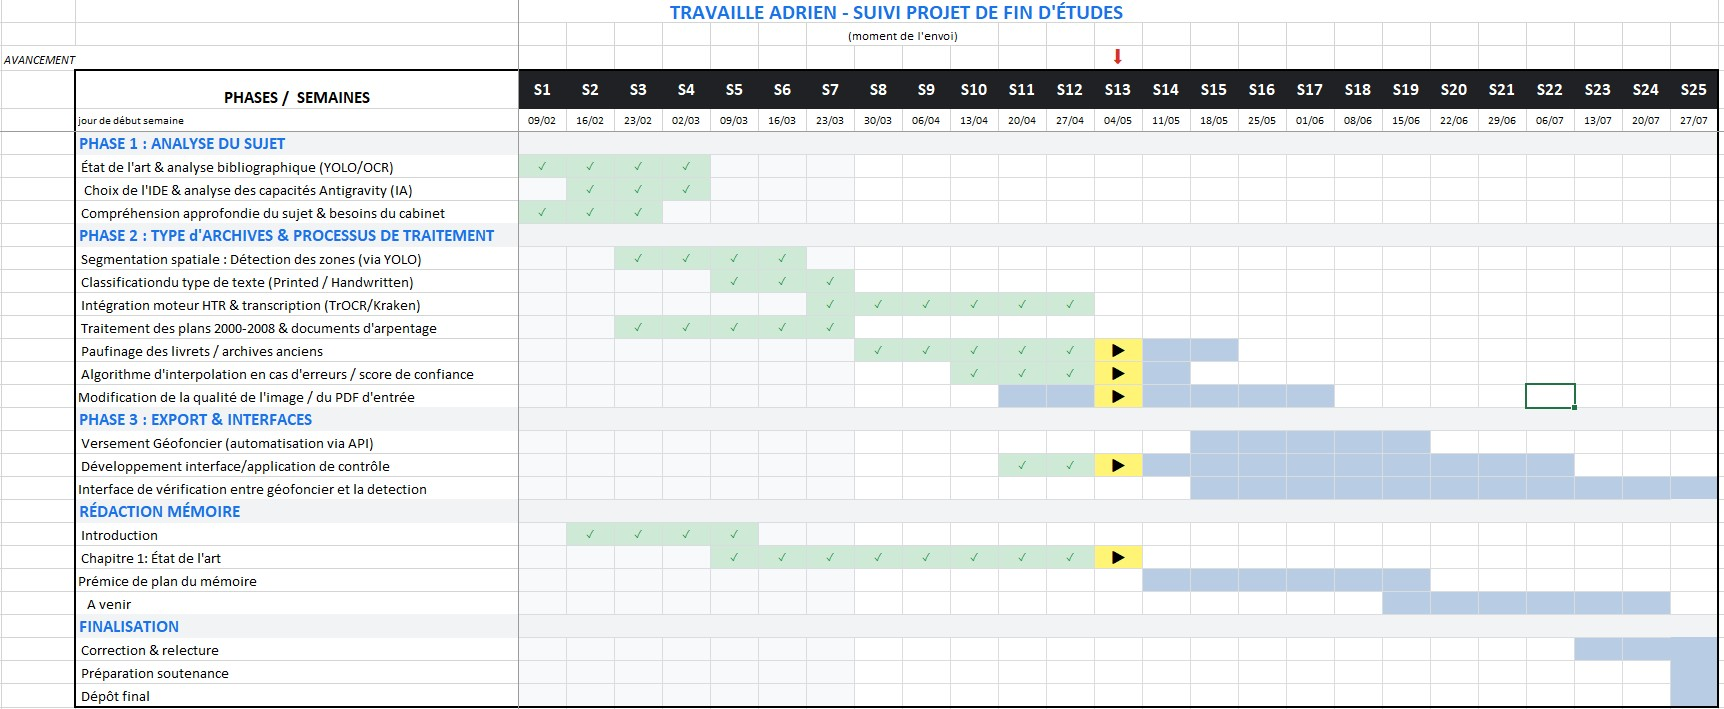
\includegraphics[width=1\textwidth]{img/planning.jpg}
  \caption{Aperçu du fichier de suivi hebdomadaire du PFE (lisible en annexe )}
  \label{fig:suivi_planning}
\end{figure}

\section{Planning prévisionnel et résultats à atteindre}
La suite du projet sera consacrée à rendre le système plus robuste notamment pour un type de livret entièrement manuel, et à préparer l'extraction sur Géofoncier. La difficulté principale restante concerne le versement final des données, notamment via les API (Application Programming Interface) présentes sur le portail des géomètres-experts.

L'objectif à terme est d'atteindre une automatisation complète. Lorsqu'une archive est lue par le système, le programme devra exécuter deux actions consécutives :
\begin{enumerate}[leftmargin=1.2em]
  \item \textbf{Création des dossiers en interne} : Un dossier physique doit être généré automatiquement à l'emplacement réseau adéquat, correspondant précisément à la commune et au numéro de parcelle identifiés.
  \item \textbf{Création de l'entité sur Géofoncier} : Le système doit communiquer avec l'API pour générer la \enquote{pastille} correspondante directement sur la carte de la plateforme.
\end{enumerate}

D'un point de vue technique, ce versement automatisé et contrôlé sur le portail Géofoncier nécessite le même format de données. Le programme devra structurer les informations validées dans un format informatique standardisé et compréhensible par les machines (le format JSON). Le script devra ensuite s'authentifier de manière sécurisée auprès des serveurs de l'Ordre des géomètres-experts (via la génération d'un jeton d'authentification ou Token) avant d'envoyer des requêtes web de type \enquote{POST}. C'est l'API de Géofoncier qui se chargera d'interpréter ces requêtes pour créer automatiquement les objets géographiques et y lier les métadonnées de l'archive (date, nom du géomètre, type de document, que le modèle d'intelligence artificielle aura extraites en amont).

Cette dernière étape exige une donnée de qualité. Si les données extraites au préalable comportent une erreur de lecture, le programme générera des dossiers mal rangés et, plus grave encore, insérera des informations erronées sur la base de données publique de Géofoncier. Par conséquent, l'enjeu majeur des prochains mois est de garantir que la lecture automatisée soit irréprochable et que l'interface de contrôle empêche toute donnée incertaine d'atteindre l'API sans validation humaine préalable.

L'avancement futur est structuré en quatre étapes, présentées dans l'organigramme ci-dessous.

\begin{center}
\begin{tikzpicture}[
  node distance=10mm and 12mm,
  box/.style={draw, rounded corners, align=left, inner sep=6pt, text width=12.5cm},
  arrow/.style={-Latex, thick}
]
\node[box] (s0) {\textbf{Situation mi-parcours}\\
Outil existant pour plans modernes, validation métier en place, interface visuelle prête, exports Excel/CSV fonctionnels.};

\node[box, below=of s0] (s1) {\textbf{Étape 1 - Fiabilisation (Mai)}\\
Réduire les erreurs sur les manuscrits très abîmés, améliorer le découpage des cases, affiner les scores de confiance pour aider l'opérateur.};
\draw[arrow] (s0) -- (s1);

\node[box, below=of s1] (s2) {\textbf{Étape 2 - Préparation au versement (Juin)}\\
Apprentissage du programme via les corrections de l'opérateur et mise en place de la création automatique de l'arborescence des dossiers locaux.};
\draw[arrow] (s1) -- (s2);

\node[box, below=of s2] (s3) {\textbf{Étape 3 - Déploiement Géofoncier (Juillet)}\\
Mise au point de l'envoi des données vers l'API Géofoncier, création automatisée des pastilles, et tests pour garantir la fiabilité des versements.};
\draw[arrow] (s2) -- (s3);

\node[box, below=of s3] (s4) {\textbf{Étape 4 - Évaluation et livraison (Fin Juillet)}\\
Mesure du gain de temps réel pour Géo-Siapp par rapport à une saisie manuelle, finalisation du mémoire.};
\draw[arrow] (s3) -- (s4);
\end{tikzpicture}
\end{center}

\addcontentsline{toc}{section}{Conclusion}
\section*{Conclusion}
À la moitié du temps d'étude, le système d'extraction des plans récents ainsi que l'interface de validation sont opérationnels. L'outil sait analyser le document, identifier les informations et les exporter. Le reste du projet portera spécifiquement sur le traitement des livrets d'archives entièrement manuscrits. L'objectif final sera d'obtenir une donnée de qualité suffisante pour permettre, de manière automatisée, la création des dossiers locaux (selon le numéro de parcelle et la commune) et le versement des informations sur le portail des géomètres-experts (Géofoncier).
\clearpage
\addcontentsline{toc}{section}{Bibliographie}
\bibliographystyle{plainnat}
\bibliography{PFE_AT}
\clearpage
\appendix
\addcontentsline{toc}{section}{Annexes}
\section*{Annexes}

\subsection{Schéma d'architecture globale }
\begin{figure}[p]
  \centering
  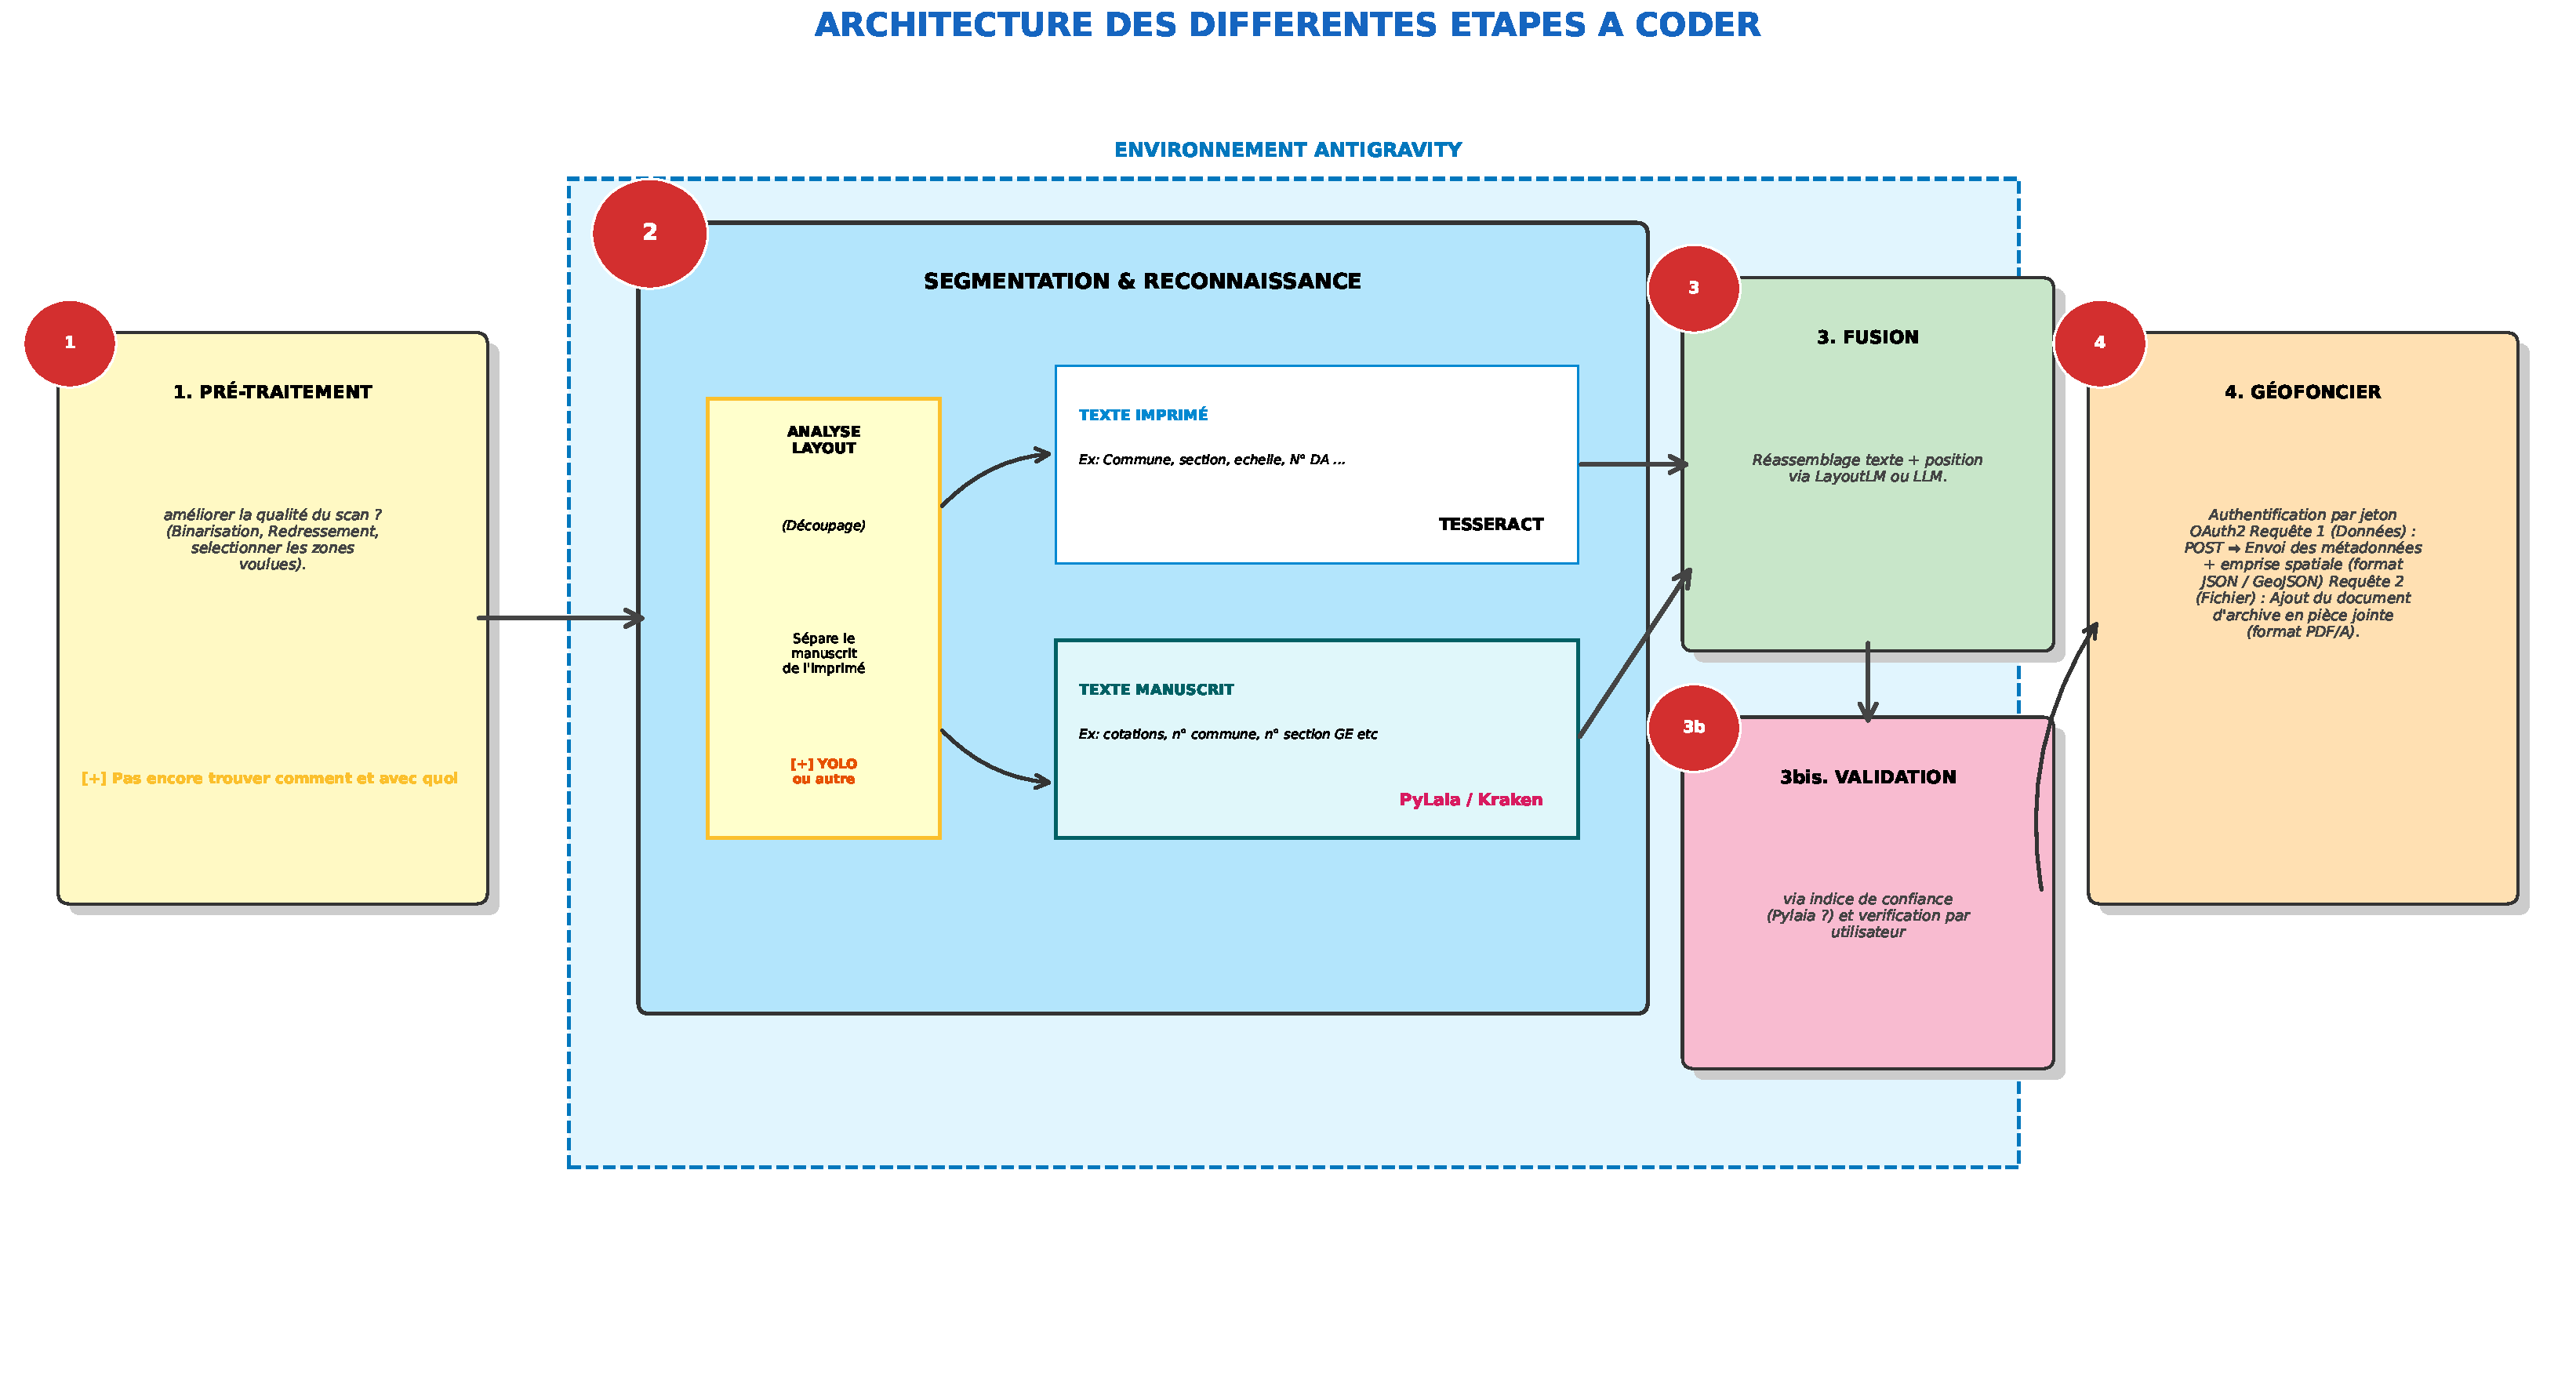
\includegraphics[width=0.95\textheight, angle=90]{img/architecture_pfe_complet.pdf}
  \caption{Vue détaillée de l'architecture globale du projet}
\end{figure}

\subsection{Planning et suivi hebdomadaire }
\begin{figure}[p]
  \centering
  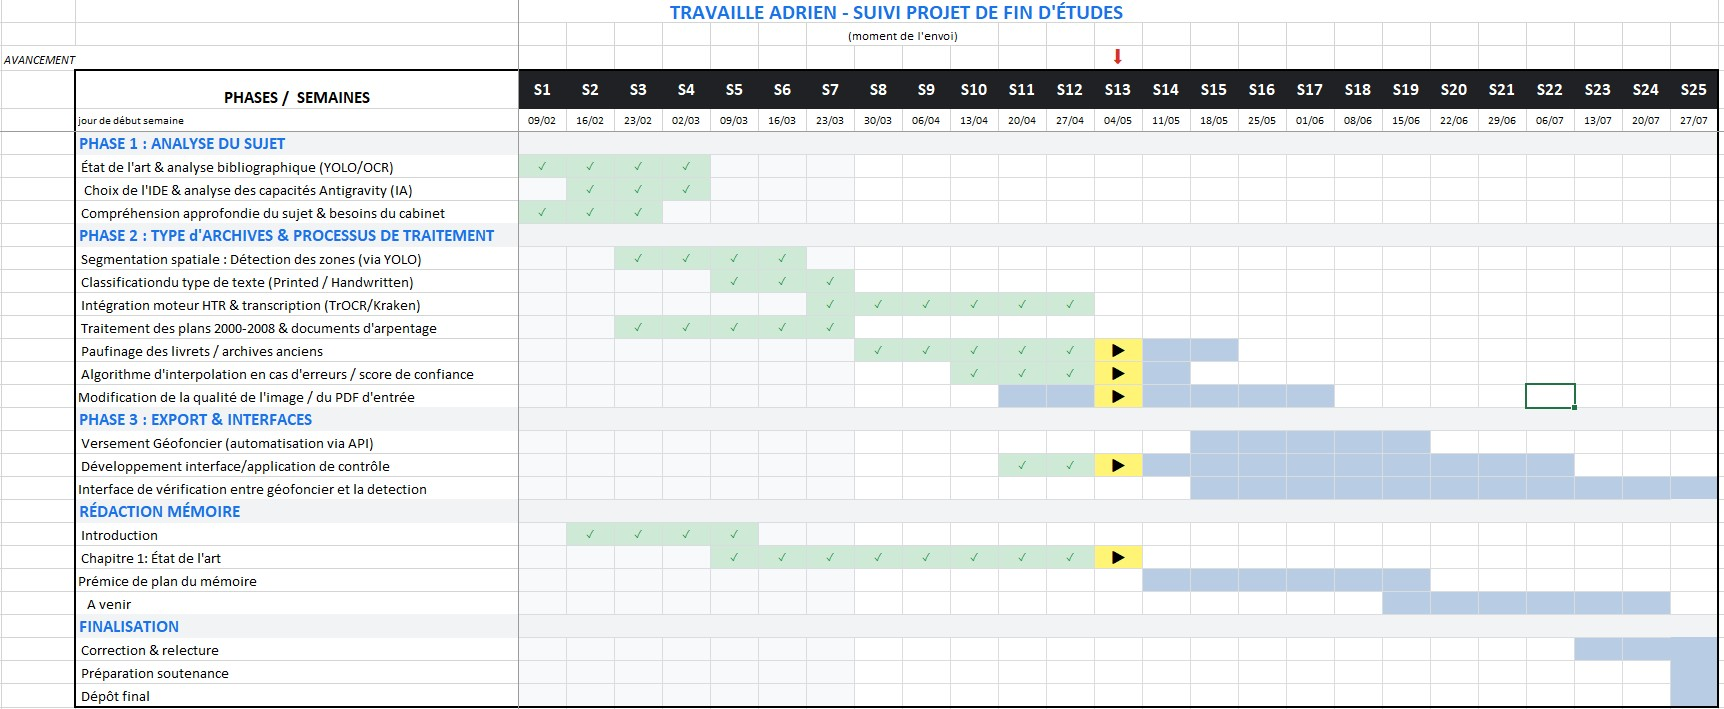
\includegraphics[width=0.95\textheight, angle=90]{img/planning.jpg}
  \caption{Vue détaillée du fichier de suivi hebdomadaire}
\end{figure}

\clearpage
\addcontentsline{toc}{section}{\listfigurename}
\listoffigures

\end{document}

